\documentclass{article} % For LaTeX2e
\usepackage{iclr2017,times}
\usepackage{hyperref}
\usepackage{url}

\usepackage[utf8]{inputenc}
\usepackage{amsmath}
\usepackage{amssymb}
\usepackage{csquotes}
\usepackage{graphicx}
\usepackage{subfigure}
\usepackage{booktabs}

%\setlength{\bibsep}{1.52pt} %comment for arxiv
%\usepackage{parskip} \setlength{\parskip}{3pt}

%\title{Spatio-Temporal Sequence-to-Sequence Modeling with Graph Convolutional Recurrent Networks}
%\title{Graph Convolutional Recurrent Network\\
%for Structured Sequence Modeling}
\title{Structured Sequence Modeling with \\ Graph Convolutional Recurrent Networks}
%\title{Structured Sequence Prediction with \\ Graph Convolutional Recurrent Networks}
%\title{Graph Convolutional Recurrent Network\\
%for Spatio-Temporal Sequence Modeling}
%\title{Graph Convolutional Recurrent Neural Network}
%\title{Graph Convolutional LSTM Network}
%\title{Graph Convolutional RNN}

%\author{Youngjoo Seo, Michaël Defferrard, Pierre Vandergheynst \\
%EPFL, Lausanne, Switzerland \\
%\texttt{\{youngjoo.seo, michael.defferrard, pierre.vandergheynst\}@epfl.ch} \\
%\And
%Xavier Bresson \\
%Nanyang Technological University, Singapore \\
%\texttt{\{xavier.bresson@ntu.edu.sg} \\
%}

\author{
Youngjoo Seo \\
EPFL, Switzerland \\
\texttt{youngjoo.seo@epfl.ch} \\
\And
Michaël Defferrard \\
EPFL, Switzerland \\
\texttt{michael.defferrard@epfl.ch} \\
\And
Pierre Vandergheynst \\
EPFL, Switzerland \\
\texttt{pierre.vandergheynst@epfl.ch} \\
\And
Xavier Bresson \\
EPFL, Switzerland \\
\texttt{xavier.bresson@epfl.ch} 
}

\newcommand{\fix}{\marginpar{FIX}}
\newcommand{\new}{\marginpar{NEW}}

\DeclareMathOperator*{\diag}{diag}
\DeclareMathOperator*{\argmin}{arg\,min}
\DeclareMathOperator*{\argmax}{arg\,max}
\DeclareMathOperator*{\spn}{span}
\newcommand{\R}{\mathbb{R}}
\newcommand{\bO}{\mathcal{O}}
\newcommand{\G}{\mathcal{G}}
\newcommand{\V}{\mathcal{V}}
\newcommand{\E}{\mathcal{E}}
\newcommand{\figref}[1]{Figure~\ref{fig:#1}}
\newcommand{\tabref}[1]{Table~\ref{tab:#1}}
\newcommand{\eqnref}[1]{(\ref{eqn:#1})}
\newcommand{\secref}[1]{Section~\ref{sec:#1}}

\usepackage{color}
\newcommand{\todo}[1]{{\color{red} #1 }}


%\iclrfinalcopy % Uncomment for camera-ready version

\begin{document}

\maketitle

\begin{abstract}
	This paper introduces Graph Convolutional Recurrent
	Network (GCRN), a deep learning model able to predict structured
	sequences of data. Precisely, GCRN is a generalization of classical recurrent neural networks (RNN) to
	data structured by an arbitrary graph. 
 	%So far the only underlying structures that have been explored in the sequence modeling literature are the linear chain, the 2D grid and the tree.
	Such structured sequences can represent series of frames in videos, spatio-temporal measurements on a network of
	sensors, or random walks on a vocabulary graph for natural language modeling.
	The proposed model combines convolutional neural networks (CNN) on graphs to identify spatial structures and RNN to find dynamic patterns. We study two possible architectures of GCRN, and apply the models to two practical
	problems: predicting moving MNIST data, and modeling natural language with the Penn
	Treebank dataset. Experiments show that exploiting simultaneously graph spatial and dynamic information about data can improve both precision and learning speed.
\end{abstract}

	

\section{Introduction}

% Motivate using the unsupervised argument ?
% LSTM have been used widely. No need, well known fact.

Many real-world data can be cast as structured sequences, with spatio-temporal
sequences being a special case. A well-studied example of spatio-temporal data are videos, where
succeeding frames share temporal and spatial structures. Many works, such as \citet{cnnlstm1, cnnlstm2, cnnlstm3},  leveraged a combination of CNN and RNN to exploit such spatial and
temporal regularities. Their models are able to process possibly time-varying
visual inputs for variable-length prediction. These neural network architectures consist of combining
a CNN for visual feature extraction followed by a RNN for sequence learning. Such
architectures have been successfully used for video activity recognition, image
captioning and video description.

More recently, interest has grown in properly fusing the CNN and RNN models for
spatio-temporal sequence modeling. Inspired by language modeling,
\citet{video_language_model} proposed a model to represent complex deformations
and motion patterns by discovering both spatial and temporal correlations. They showed that prediction of the next video frame and
interpolation of intermediate frames can be achieved by building a RNN-based
language model on the visual words obtained by quantizing the image patches.
Their highest-performing model, recursive CNN (rCNN), uses convolutions for both
 inputs and states. \citet{convlstm}  then proposed the convolutional
LSTM network (convLSTM), a recurrent model for spatio-temporal sequence
modeling which uses 2D-grid convolution to leverage the spatial correlations in
input data. They successfully applied their model to the prediction of the
evolution of radar echo maps for precipitation nowcasting.

% \todo{speak about seq2seq}

% \citet{moving_mnist} build on that work and points out the importance of
% multi-step prediction in learning useful representations. They build an LSTM
% encoder-decoder-predictor model which reconstructs the input sequence and
% predicts the future sequence simultaneously. The \textit{fully connected}
% LSTM (FC-LSTM) layer adopted by them does however not encode spatial
% relations. 

The spatial structure of many important problems may however not be as simple as regular grids. For instance, 
the data measured from meteorological stations lie on a irregular grid, i.e. a network of heterogeneous spatial
distribution of stations. More challenging, the spatial structure of data may not even be spatial, as it is the case for social or biological networks. Eventually, the interpretation that sentences can be regarded as random walks on vocabulary graphs,
a view popularized by \cite{word2vec}, allows us to cast language analysis problems as graph-structured sequence models.

This work leverages on the recent models of \cite{gcnn,video_language_model,convlstm} to design the GCRN model for modeling and predicting time-varying graph-based data. The core idea is to merge CNN for graph-structured data and RNN to identify simultaneously meaningful spatial structures and dynamic patterns. A generic illustration of the proposed GCRN architecture is given by Figure \ref{fig1}.


\begin{figure}[ht]
	\centering
	%\framebox[4.0in]{$\;$}
	%\fbox{\rule[-.5cm]{0cm}{5cm} \rule[-.5cm]{\linewidth}{0cm}}
	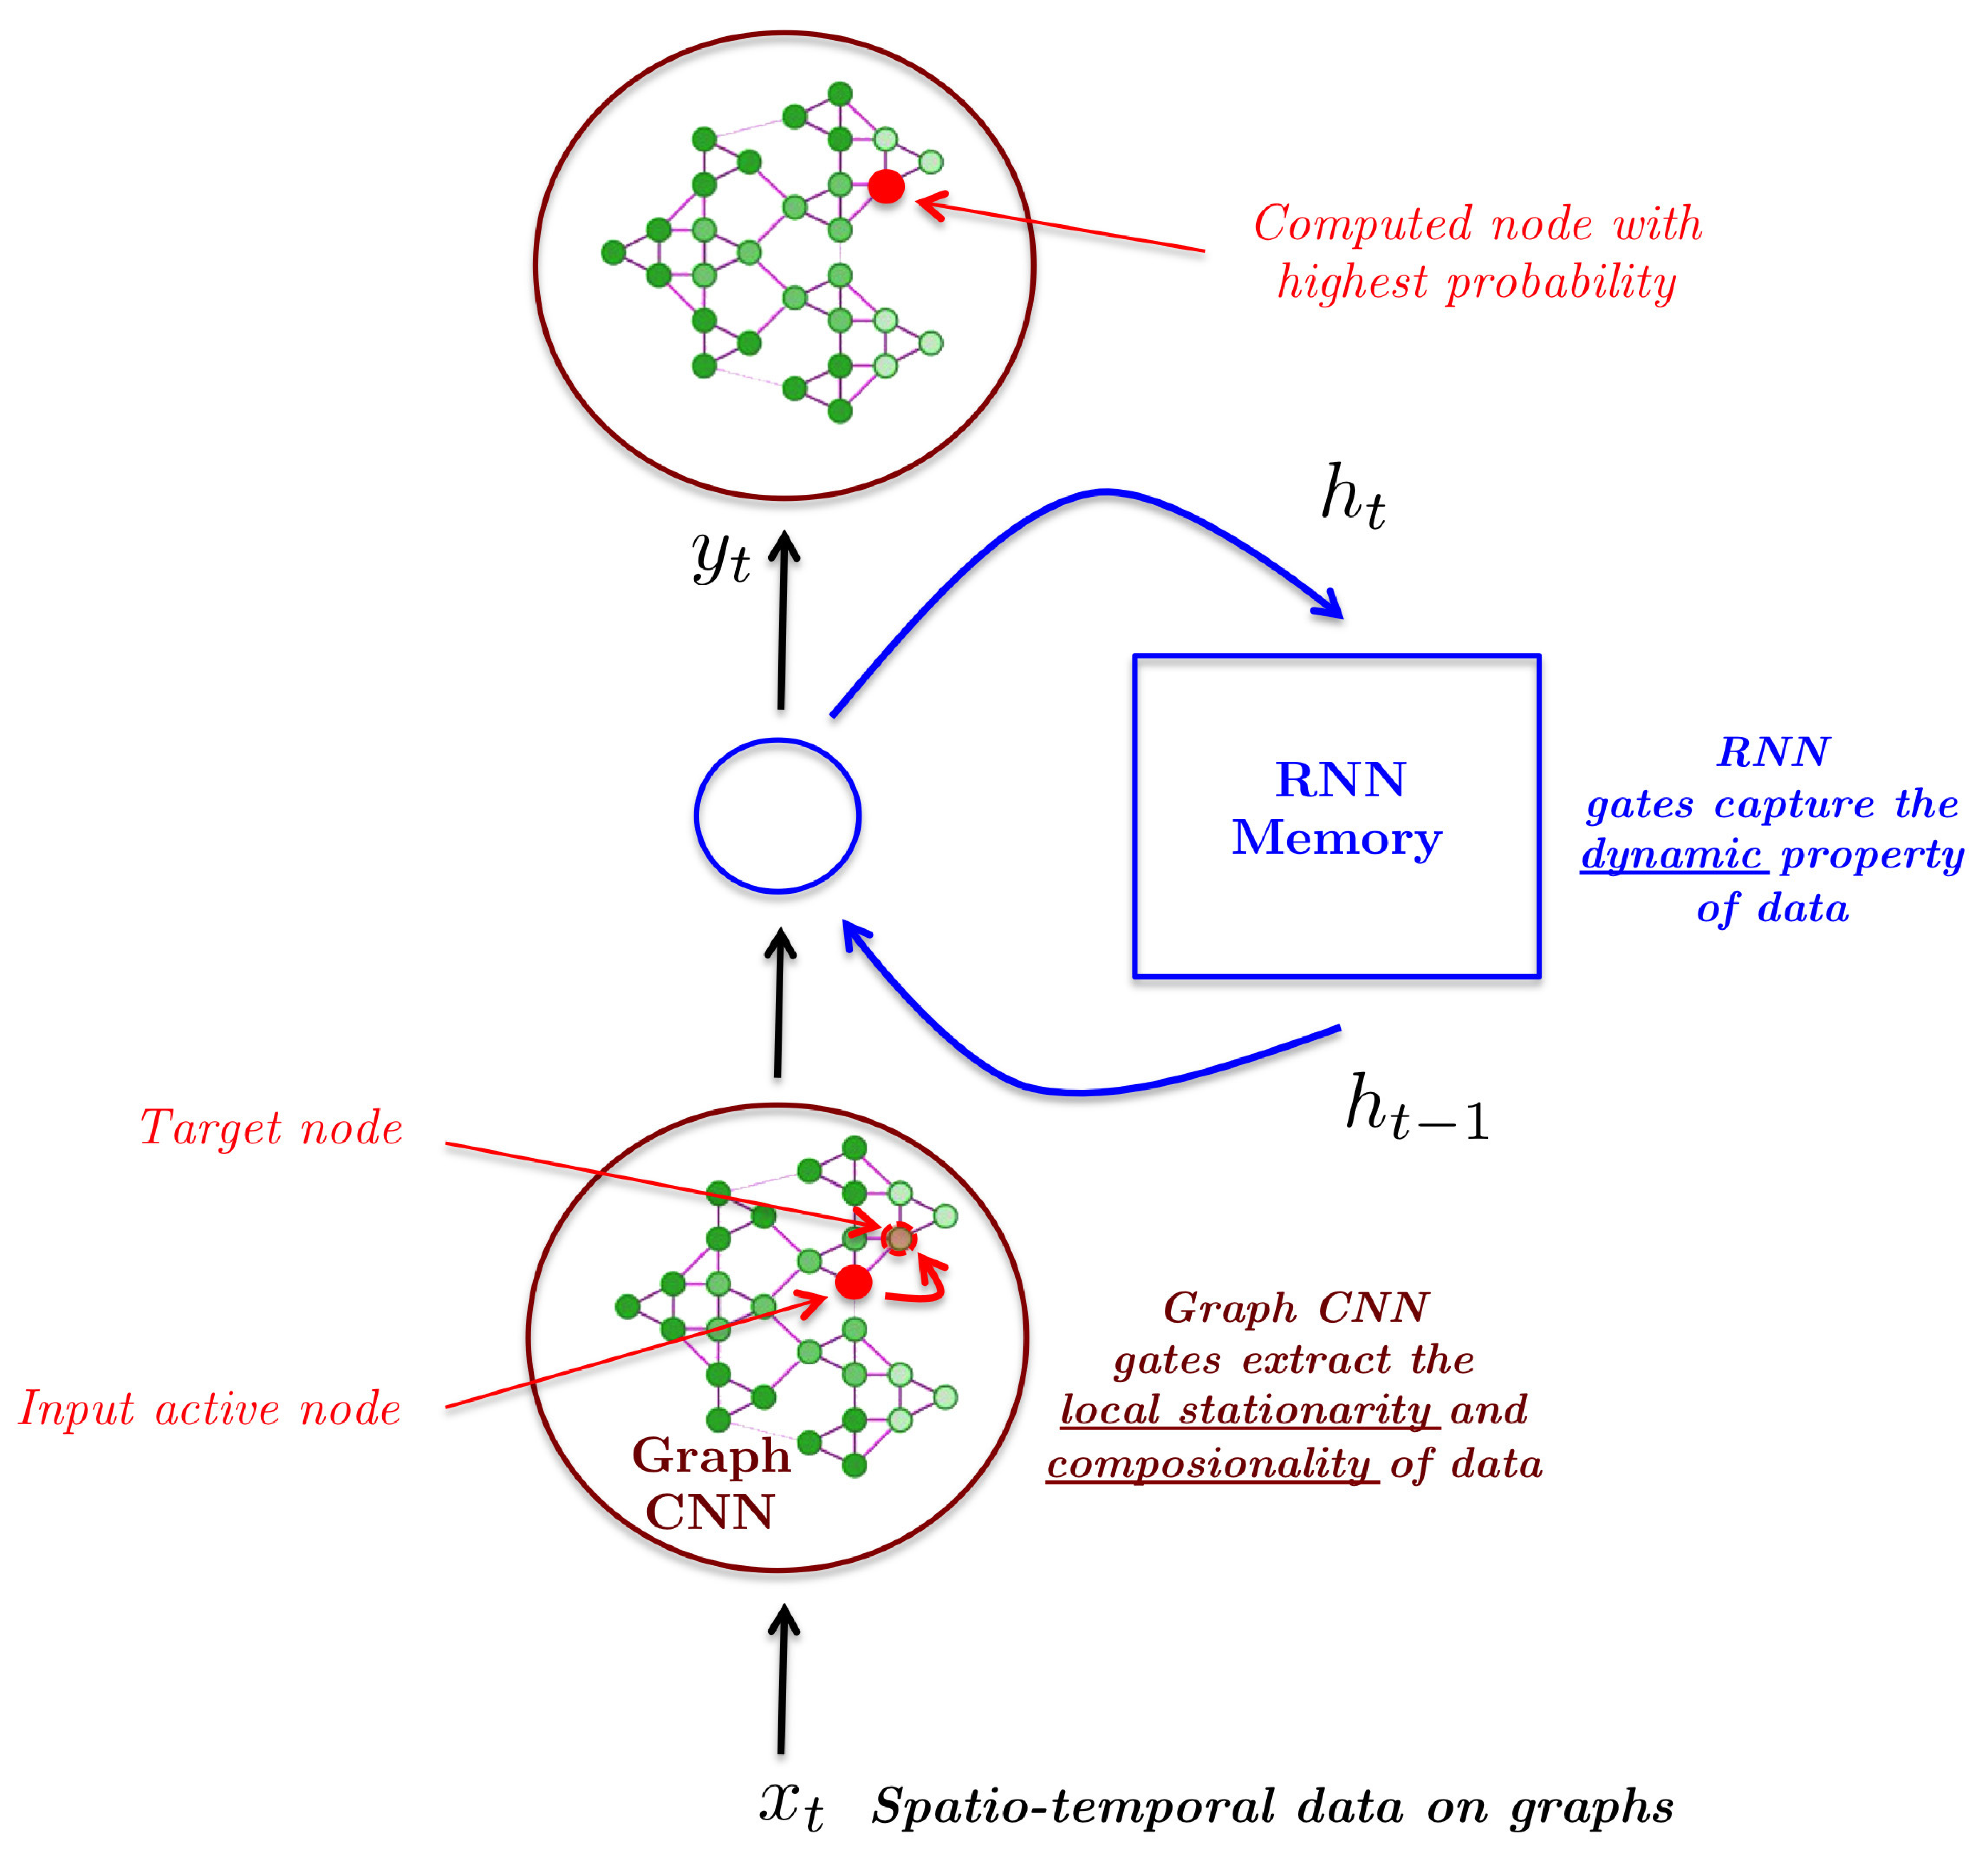
\includegraphics[width=10cm]{figures/gcnn_rnn.pdf}
	\caption{Illustration of the proposed GCRN model for spatio-temporal prediction of graph-structured data. The technique combines at the same time CNN on graphs and RNN. RNN can be easily exchanged with LSTM or GRU networks.} 
	\label{fig1}
\end{figure}



%\begin{figure}[t]
%	\centering
%	%\framebox[4.0in]{$\;$}
%	\fbox{\rule[-.5cm]{0cm}{5cm} \rule[-.5cm]{\linewidth}{0cm}}
%	\caption{\todo{Comparison: linear, tree, graph 1-neighborhood, graph conv}}
%\end{figure}

% capture statistical properties in the joint domain

\section{Preliminaries}

% This section introduces the three building blocks our work relies on: (i) the
% structured sequence modeling problem, (ii) LSTM networks and (iii)
% convolutional neural networks defined on graphs.

\subsection{Structured Sequence Modeling}

Sequence modeling is the problem of predicting the most likely future
length-$K$ sequence given the previous $J$ observations:
\begin{equation} \label{eqn:seq}
	\hat{x}_{t+1}, \ldots, \hat{x}_{t+K} =
	\argmax_{x_{t+1}, \ldots, x_{t+K}}
	P(x_{t+1}, \ldots, x_{t+K} | x_{t-J+1}, \ldots, x_t),
\end{equation}
where $x_t \in \mathbf{D}$ is an observation at time $t$ and $\mathbf{D}$
denotes the domain of the observed features. The archetypal application being
the $n$-gram language model (with $n = J+1$), where $P(x_{t+1} | x_{t-J+1},
\ldots, x_t)$ models the probability of word $x_{t+1}$ to appear conditioned on
the past $J$ words in the sentence \citep{seq_graves}.

In this paper, we are interested in special structured sequences, i.e. sequences where features of the observations $x_t$ are not independent but linked by pairwise relationships. Such relationships are universally modeled by weighted graphs. 

Data $x_t$ can be viewed as a graph signal, i.e.
a signal defined on an undirected and weighted graph $\G = (\V, \E, A)$, where
$\V$ is a finite set of $|\V| = n$ vertices, $\E$ is a set of edges and $A \in
\R^{n \times n}$ is a weighted adjacency matrix encoding the connection weight
between two vertices. A signal $x_t: \V \rightarrow \R^{d_x}$ defined on the
nodes of the graph may be regarded as a matrix $x_t \in \R^{n \times d_x}$
whose column $i$ is the $d_x$-dimensional value of $x_t$ at the $i^{th}$ node.
While the number of free variables in a structured sequence of length $K$ is in
principle $\bO(n^K {d_x}^K)$, we seek to exploit the structure of the space
of possible predictions to reduce the dimensionality and hence make those
problems more tractable.

\subsection{Long Short-Term Memory}

% Leaving the structure apart, a structured sample could be processed by a classical LSTM.

A special class of recurrent neural networks (RNN) that prevents the gradient from vanishing
too quickly is the popular long short-term memory (LSTM) introduced by \citet{lstm}. This architecture has proven stable and powerful for modeling long-range dependencies in various general-purpose sequence modeling tasks
\citep{seq_graves, moving_mnist, seq2seq}. A fully-connected LSTM (FC-LSTM) may
be seen as a multivariate version of LSTM where the input $x_t \in \R^{d_x}$,
cell output $h_t \in [-1,1]^{d_h}$ and states $c_t \in \R^{d_h}$ are all
vectors. In this paper, we follow the FC-LSTM formulation of
\citet{seq_graves}, that is:
\begin{align} \label{eqn:lstm_fc}
\begin{split}
	i &= \sigma(W_{xi} x_t + W_{hi} h_{t-1} + w_{ci} \odot c_{t-1} + b_i), \\
	f &= \sigma(W_{xf} x_t + W_{hf} h_{t-1} + w_{cf} \odot c_{t-1} + b_f), \\
	c_t &= f_t \odot c_{t-1} + i_t \odot \tanh(W_{xc} x_t + W_{hc} h_{t-1} + b_c), \\
	o &= \sigma(W_{xo} x_t + W_{ho} h_{t-1} + w_{co} \odot c_t + b_o), \\
	h_t &= o \odot \tanh(c_t),
\end{split}
\end{align}
where $\odot$ denotes the Hadamard product, $\sigma(\cdot)$ the sigmoid
function $\sigma(x) = 1 / (1+e^{-x})$ and $i, f, o \in [0,1]^{d_h}$ are the
input, forget and output gates. The weights $W_{x\cdot} \in \R^{d_h \times
d_x}$, $W_{h\cdot} \in \R^{d_h \times d_h}$, $w_{c\cdot} \in \R^{d_h}$ and
biases $b_i, b_f, b_c, b_o \in \R^{d_h}$ are the model parameters.\footnote{A
practical trick is to initialize the biases $b_i$, $b_f$ and $b_o$ to one such
that the gates are initially open.} Such a model is called fully-connected
because the dense matrices $W_{x\cdot}$ and $W_{h\cdot}$ linearly combine all
the components of $x$ and $h$. The optional peephole connections $w_{c\cdot}
\odot c_t$, introduced by \citet{peephole}, have been found to improve
performance on certain tasks.

%The major innovation of LSTM resides in the introduction of the memory cell
%$c_t$ and the various gates, which together control the flow of information
%and allows the gradient to be trapped in the cell.

\subsection{Convolutional Neural Networks on Graphs} \label{sec:graphconv}

Generalizing convolutional neural networks (CNNs) to arbitrary graphs is a
recent area of interest. Two approaches have been explored in the literature: (i) a
generalization of the spatial definition of a convolution \citep{gcnn_masci,
gcnn_niepert} and (ii), a multiplication in the graph Fourier domain by the way
of the convolution theorem \citep{gcnn_bruna, gcnn}. \citet{gcnn_masci}
introduced a spatial generalization of CNNs to 3D meshes. The authors used
geodesic polar coordinates to define convolution operations on mesh patches,
and formulated a deep learning architecture which allows comparison across
different meshes.  Hence, this method is tailored to manifolds and is not directly
generalizable to arbitrary graphs. \citet{gcnn_niepert} proposed a spatial
approach which may be decomposed in three steps: (i) select a node, (ii)
construct its neighborhood and (iii) normalize the selected sub-graph, i.e.
order the neighboring nodes. The extracted patches are then fed into a
conventional 1D Euclidean CNN. As graphs generally do not possess a natural ordering
(temporal, spatial or otherwise), a labeling procedure should be used to impose
it. \citet{gcnn_bruna} were the first to introduce the spectral framework
described below in the context of graph CNNs. The major drawback of this
method is its $\bO(n^2)$ complexity, which was overcome with the technique of \citet{gcnn}, which offers a linear complexity $\bO(|\E|)$ and provides strictly localized
filters. \citet{gcnn_kipf} took a first-order approximation of the spectral
filters proposed by \citet{gcnn} and successfully used it for semi-supervised
classification of nodes. While we focus on the framework introduced by
\citet{gcnn}, the proposed model is agnostic to the choice of the graph
convolution operator $\ast_\G$. % \todo{atwood, duvenaud ?}

As it is difficult to express a meaningful translation operator in the vertex
domain \citep{gcnn_bruna, gcnn_niepert}, \citet{gcnn} chose a spectral
formulation for the convolution operator on graph $\ast_\G$. By this
definition, a graph signal $x \in \R^{n \times d_x}$ is filtered by a non-parametric kernel
$g_\theta(\Lambda) = \diag(\theta)$, where $\theta \in \R^n$ is a vector of
Fourier coefficients, as
%\begin{equation}
%	x \ast_\G y = U((U^Tx) \odot (U^Ty)),
%\end{equation}
\begin{equation} \label{eqn:graph_conv}
	y = g_\theta \ast_\G x = g_\theta(L) x =
	g_\theta(U \Lambda U^T) x = U g_\theta(\Lambda) U^T x \in \R^{n \times d_x},
\end{equation}
where $U \in \R^{n \times n}$ is the matrix of eigenvectors and $\Lambda \in
\R^{n \times n}$ the diagonal matrix of eigenvalues of the normalized graph
Laplacian $L = I_n - D^{-1/2} A D^{-1/2} = U \Lambda U^T \in \R^{n \times n}$,
where $I_n$ is the identity matrix and $D \in \R^{n \times n}$ is the diagonal
degree matrix with $D_{ii} = \sum_j A_{ij}$ \citep{chung}.  Note that the
signal $x$ is filtered by $g_\theta$ with an element-wise multiplication of its
graph Fourier transform $U^T x$ with $g_\theta$ \citep{gsp}. Evaluating
\eqnref{graph_conv} is however expensive, as the multiplication with $U$ is
$\bO(n^2)$. Furthermore, computing the eigendecomposition of $L$ might be
prohibitively expensive for large graphs. To circumvent this problem,
\cite{gcnn} parametrizes $g_\theta$ as a truncated expansion, up to order
$K-1$, of Chebyshev polynomials $T_k$ such that
\begin{equation} \label{eqn:filt_cheby}
	g_\theta(\Lambda) = \sum_{k=0}^{K-1} \theta_k T_k(\tilde{\Lambda}),
\end{equation}
where the parameter $\theta \in \R^K$ is a vector of Chebyshev coefficients and
$T_k(\tilde{\Lambda}) \in \R^{n \times n}$ is the Chebyshev polynomial of order
$k$ evaluated at $\tilde{\Lambda} = 2 \Lambda / \lambda_{max} - I_n$. The
graph filtering operation can then be written as
\begin{equation} \label{eqn:graph_conv_cheby}
	y = g_\theta \ast_\G x = g_\theta(L) x = \sum_{k=0}^{K-1} \theta_k T_k(\tilde{L}) x,
\end{equation}
where $T_k(\tilde{L}) \in \R^{n \times n}$ is the Chebyshev polynomial of order
$k$ evaluated at the scaled Laplacian $\tilde{L} = 2 L / \lambda_{max} - I_n$.
Using the stable recurrence relation $T_k(x) = 2x T_{k-1}(x) - T_{k-2}(x)$ with
$T_0 = 1$ and $T_1 = x$, one can evaluate \eqnref{graph_conv_cheby} in
$\bO(K|\E|)$ operations, i.e. linearly with the number of edges. Note that as
the filtering operation \eqnref{graph_conv_cheby} is an order $K$ polynomial of
the Laplacian, it is $K$-localized and depends only on nodes that are at
maximum $K$ hops away from the central node, the $K$-neighborhood. The reader
is referred to \cite{gcnn} for details and an in-depth discussion.

\section{Related Works}

%\paragraph{Spatio-temporal sequence modeling with a combination of recurrent nets and convolutions.}
%\paragraph{Convolutional LSTM (convLSTM).} 
%\paragraph{Recurrent convolutional neural network (rCNN).}
%\paragraph{Non-convolutional approaches.}

\citet{convlstm} introduced a model for regular grid-structured sequences, which can be
seen as a special case of the proposed model where the graph is an image grid where the
nodes are well ordered. Their model is essentially the classical FC-LSTM
\eqnref{lstm_fc} where the multiplications by dense matrices $W$ have been
replaced by convolutions with kernels $W$:
\begin{align} \label{eqn:lstm_conv}
\begin{split}
	i &= \sigma(W_{xi} \ast x_t + W_{hi} \ast h_{t-1} +
	            w_{ci} \odot c_{t-1} + b_i), \\
	f &= \sigma(W_{xf} \ast x_t + W_{hf} \ast h_{t-1} +
	            w_{cf} \odot c_{t-1} + b_f), \\
	c_t &= f_t \odot c_{t-1} + i_t \odot
	       \tanh(W_{xc} \ast x_t + W_{hc} \ast h_{t-1} + b_c), \\
	o &= \sigma(W_{xo} \ast x_t + W_{ho} \ast h_{t-1} +
	            w_{co} \odot c_t + b_o), \\
	h_t &= o \odot \tanh(c_t),
\end{split}
\end{align}
where $\ast$ denotes the 2D convolution by a set of kernels. In their setting,
the input tensor $x_t \in \R^{n_r \times n_c \times d_x}$ is the observation of
$d_x$ measurements at time $t$ of a dynamical system over a spatial region
represented by a grid of $n_r$ rows and $n_c$ columns. The model holds
spatially distributed hidden and cell states of size $d_h$ given by the tensors
$c_t, h_t \in \R^{n_r \times n_c \times d_h}$. The size $m$ of the
convolutional kernels $W_{h\cdot} \in \R^{m \times m \times d_h \times d_h}$
and $W_{x\cdot} \in \R^{m \times m \times d_h \times d_x}$ determines the
number of parameters, which is independent of the grid size $n_r \times n_c$.
Earlier, \citet{video_language_model} proposed a similar RNN variation which
uses convolutional layers instead of fully connected layers. The hidden state
at time $t$ is given by
\begin{equation}
	h_t = \tanh(\sigma(W_{x2} \ast \sigma(W_{x1} \ast x_t)) + \sigma(W_h \ast h_{t-1})),
\end{equation}
where the convolutional kernels $W_h \in \R^{d_h \times d_h}$ are restricted to
filters of size 1x1 (effectively a fully connected layer shared across all
spatial locations).

Observing that natural language exhibits syntactic properties that naturally
combine words into phrases, \citet{treelstm} proposed a model for
tree-structured topologies, where each LSTM has access to the states of its
children. They obtained state-of-the-art results on semantic relatedness and
sentiment classification. \citet{graphlstm} followed up and proposed a variant
on graphs. Their sophisticated network architecture obtained state-of-the-art
results for semantic object parsing on four datasets. In those models, the
states are gathered from the neighborhood by way of a weighted sum with
trainable weight matrices. Those weights are however not shared across the
graph, which would otherwise have required some ordering of the nodes, alike
any other spatial definition of graph convolution. Moreover, their formulations
are limited to the one-neighborhood of the current node, with equal weight
given to each neighbor.

Motivated by spatio-temporal problems like modeling human motion and object
interactions, \citet{structuralrnn} developed a method to cast a
spatio-temporal graph as a rich RNN mixture which essentially associates a RNN
to each node and edge. Again, the communication is limited to directly
connected nodes and edges.

% \citet{deepstruct} combined Markov random fields with deep learning

\citet{ggsnn_li} proposed a similar model based on the propagation rule of
\citet{gnn_scarcelli}. They showed stat-of-the-art on a problem from program
verification.

\section{Proposed GCRN Models}
\label{sec:our_models}

% Two models:
% 1. conv output to vRNN / LSTM
% 2. integrating conv and LSTM

We propose two GCRN architectures that are quite natural, and investigate their performances in real-world applications in Section \ref{experiments}.


{\it Model 1.} We first consider a natural end-to-end learning system, meaning that we stack a graph CNN, defined as
\eqnref{graph_conv_cheby}, for feature extraction and a LSTM, defined as \eqnref{lstm_fc}, for sequence learning: \begin{align} \label{eqn:lstm_graph_v1}
\begin{split}
	x_t^{\textrm{CNN}} &=  \textrm{CNN}_\G(x_t)\\
	i &= \sigma(W_{xi} x_t^{\textrm{CNN}} + W_{hi} h_{t-1}  +
	            w_{ci} \odot c_{t-1} + b_i), \\
	f &= \sigma(W_{xf} x_t^{\textrm{CNN}} + W_{hf} h_{t-1} + w_{cf} \odot c_{t-1} + b_f), \\
	c_t &= f_t \odot c_{t-1} + i_t \odot \tanh(W_{xc} x_t^{\textrm{CNN}} + W_{hc} h_{t-1} + b_c), \\
	o &= \sigma(W_{xo} x_t^{\textrm{CNN}} + W_{ho} h_{t-1} + w_{co} \odot c_t + b_o), \\
	h_t &= o \odot \tanh(c_t).
\end{split}
\end{align}
In that setting, the input matrix $x_t \in \R^{n \times d_x}$ may represent the
observation of $d_x$ measurements at time $t$ of a dynamical system over a
network whose organization is given by a graph $\G$. $x_t^{\textrm{CNN}}$ is the output of the graph CNN gate. For a proof of concept, we simply choose here $x_t^{\textrm{CNN}} = W^{\textrm{CNN}} \ast_\G x_t$, where $W^{\textrm{CNN}} \in \R^{K \times d_x \times d_x}$ are the Chebyshev coefficients  for the graph convolutional kernels of support $K$. The model also holds spatially distributed hidden and cell states of size $d_h$ given by the matrices $c_t, h_t \in \R^{n \times d_h}$. Peepholes are controlled by $w_{c\cdot} \in \R^{n \times d_h}$. The weights $W_{h\cdot} \in
\R^{ d_h \times d_h}$ and $W_{x\cdot} \in \R^{d_h \times d_x}$ are the parameters of the fully connected layers. An architecture such as \eqnref{lstm_graph_v1} may be enough to capture the data distribution by exploiting local stationarity and compositionality properties as well as the dynamic properties.

% Similarly to \citet{video_language_model, convlstm}
{\it Model 2.} We generalize the convLSTM model \eqnref{lstm_conv} to graphs by simply 
replacing the Euclidean 2D convolution $\ast$ by the graph convolution
$\ast_\G$:
\begin{align} \label{eqn:lstm_graph_v2}
\begin{split}
	i &= \sigma(W_{xi} \ast_\G x_t + W_{hi} \ast_\G h_{t-1} +
	            w_{ci} \odot c_{t-1} + b_i), \\
	f &= \sigma(W_{xf} \ast_\G x_t + W_{hf} \ast_\G h_{t-1} +
	            w_{cf} \odot c_{t-1} + b_f), \\
	c_t &= f_t \odot c_{t-1} + i_t \odot
	       \tanh(W_{xc} \ast_\G x_t + W_{hc} \ast_\G h_{t-1} + b_c), \\
	o &= \sigma(W_{xo} \ast_\G x_t + W_{ho} \ast_\G h_{t-1} +
	            w_{co} \odot c_t + b_o), \\
	h_t &= o \odot \tanh(c_t).
\end{split}
\end{align}
In that setting, the support $K$ of the graph convolutional kernels defined by
the Chebyshev coefficients $W_{h\cdot} \in \R^{K \times d_h \times d_h}$ and
$W_{x\cdot} \in \R^{K \times d_h \times d_x}$ determines the number of
parameters, which is independent of the number of nodes $n$.  To keep the
notation simple, we write $W_{xi} \ast_\G x_t$ to mean a graph convolution of
$x_t$ with $d_h d_x$ filters which are functions of the graph Laplacian $L$
parametrized by $K$ Chebyshev coefficients, as noted in \eqnref{filt_cheby} and
\eqnref{graph_conv_cheby}. In a distributed computing setting, $K$ controls
the communication overhead, i.e. the number of nodes any given node $i$ should
exchange with in order to compute its local states.

The proposed blend of RNNs and graph CNNs is not limited to LSTMs and is
straightforward to apply to any kind of recursive networks. For example, a
vanilla RNN $h_t = \tanh(W_x x_{t} + W_h h_{t-1})$ would be modified as
\begin{equation} \label{eqn:vrnn_graph}
	h_t = \tanh(W_x \ast_\G x_t + W_h \ast_\G h_{t-1}),
\end{equation}
and a Gated Recurrent Unit (GRU) \citep{gru} as
\begin{align} \label{eqn:gru_graph}
\begin{split}
	z &= \sigma(W_{xz} \ast_\G x_t + W_{hz} \ast_\G h_{t-1}), \\
	r &= \sigma(W_{xr} \ast_\G x_t + W_{hr} \ast_\G h_{t-1}), \\
	\tilde{h} &= \tanh(W_{xh} \ast_\G x_t + W_{hh} \ast_\G (r \odot h_{t-1})), \\
	h_t &= z \odot h_{t-1} + (1-z) \odot \tilde{h}.
\end{split}
\end{align}

As demonstrated by \citet{convlstm}, structure-aware LSTM cells can be stacked
and used as sequence-to-sequence models using an architecture composed of an
encoder, which processes the input sequence, and a decoder, which generates an
output sequence. A standard practice for machine translation using RNNs
\citep{gru, seq2seq}.




\section{Experiments}
\label{experiments}


\subsection{Spatio-Temporal Sequence Modeling on Moving-MNIST}

For this synthetic experiment, we use the moving-MNIST dataset generated by
\citet{convlstm}. All sequences are 20 frames long (10 frames as input and 10
frames for prediction) and contain two handwritten digits bouncing inside a $64
\times 64$ patch. Following their experimental setup, all models are trained by
minimizing the binary cross-entropy loss using back-propagation through time (BPTT)
and RMSProp with a learning rate of $10^{-3}$ and a decay rate of 0.9. We choose the best model with early-stopping on validation dataset. All
implementations are based on their Theano code and
dataset.\footnote{\url{http://www.wanghao.in/code/SPARNN-release.zip}} For the construction of the graph, we use a Euclidean distance of pixel location and connecting each pixel as a node with their K-nearest neighbors. For the fair comparison with \citep{convlstm}, we launched our experiment with {\it Model2} which is same, except for changing the convolutional operator to graph convolution $\ast_\G$. In addition, we conducted an additional experiment on rotational moving-MNIST which has rotation property that handwritten digits are rotating while they move around inside an image. 
% Also, we perform early-stopping on the validation set.

%\begin{table}
%	\centering
%	\begin{tabular}{lccccc}
%		\toprule
%		Architecture & Support & Parameters & Running time & Validation & Test\\
%		\midrule
%		FC-LSTM & N/A & 142,667,776 & N/A & - & 4832 (-)\\
%		LSTM+CNN & $5 \times 5$ & 13,524,496 & 2.10 & 3841 (4290)& 3851 (4339)\\
%		LSTM+CNN & $9 \times 9$ & 43,802,128 & 6.10 & 3899 & 3903 \\
%		LSTM+GCNN & $K=3$ & 1,629,712 & 0.82 & 3877 (4313)& 3866 (4367)\\
%		LSTM+GCNN & $K=5$ & 2,711,056 & 1.53 & 3491 (3889)& 3495 (3932)\\
%		LSTM+GCNN & $K=7$ & 3,792,400 & 1.75 & {\bf 3399 (3777)}& {\bf 3400 (3803)}\\
%		LSTM+GCNN & $K=9$ & 4,873,744 & 2.15 & 3395 (3798) & 3395 (3814)\\
%		\bottomrule
%	\end{tabular}
%	\caption{Comparison between models. Time spending per each mini-batch is written in Running time(sec). Cross-entropy of FC-LSTM is taken from \cite{convlstm} and the numbers in parenthesis refer to cross-entropy on rotational moving-MNIST. LSTM-GCNN is Model 2 defined in \eqnref{lstm_graph_v2} with 8-nearest neighbor graph.}
%	\label{tab:moving_mnist}
%\end{table}
\begin{table}
	\centering
	\begin{tabular}{lcccccc}
		\toprule
		Architecture & Support & Parameters & Running time & Test(w/o Rot) & Test(Rot) & Gap\\
		\midrule
		FC-LSTM & N/A & 142,667,776 & N/A & 4832 & - & -\\
		LSTM+CNN & $5 \times 5$ & 13,524,496 & 2.10 & 3851 & 4339 & 488 \\
		LSTM+CNN & $9 \times 9$ & 43,802,128 & 6.10 & 3903 & - & - \\
		LSTM+GCNN & $K=3$ & 1,629,712 & 0.82 & 3866 & 4367 & 501 \\
		LSTM+GCNN & $K=5$ & 2,711,056 & 1.53 & 3495 & 3932 & 437 \\
		LSTM+GCNN & $K=7$ & 3,792,400 & 1.75 & {\bf 3400} & {\bf 3803} & {\bf 403}\\
		LSTM+GCNN & $K=9$ & 4,873,744 & 2.15 & 3395 & 3814 & 419 \\
		\bottomrule
	\end{tabular}
	\caption{Comparison between models. Time spending per each mini-batch is written in Running time(sec). Cross-entropy of FC-LSTM is taken from \cite{convlstm} and the numbers in parenthesis refer to cross-entropy on rotational moving-MNIST. LSTM-GCNN is Model 2 defined in \eqnref{lstm_graph_v2} with 8-nearest neighbor graph.}
	\label{tab:moving_mnist}
\end{table}
%\begin{figure}[ht]
%	\centering
%	%\framebox[4.0in]{$\;$}
%	%\fbox{\rule[-.5cm]{0cm}{5cm} \rule[-.5cm]{\linewidth}{0cm}}
%	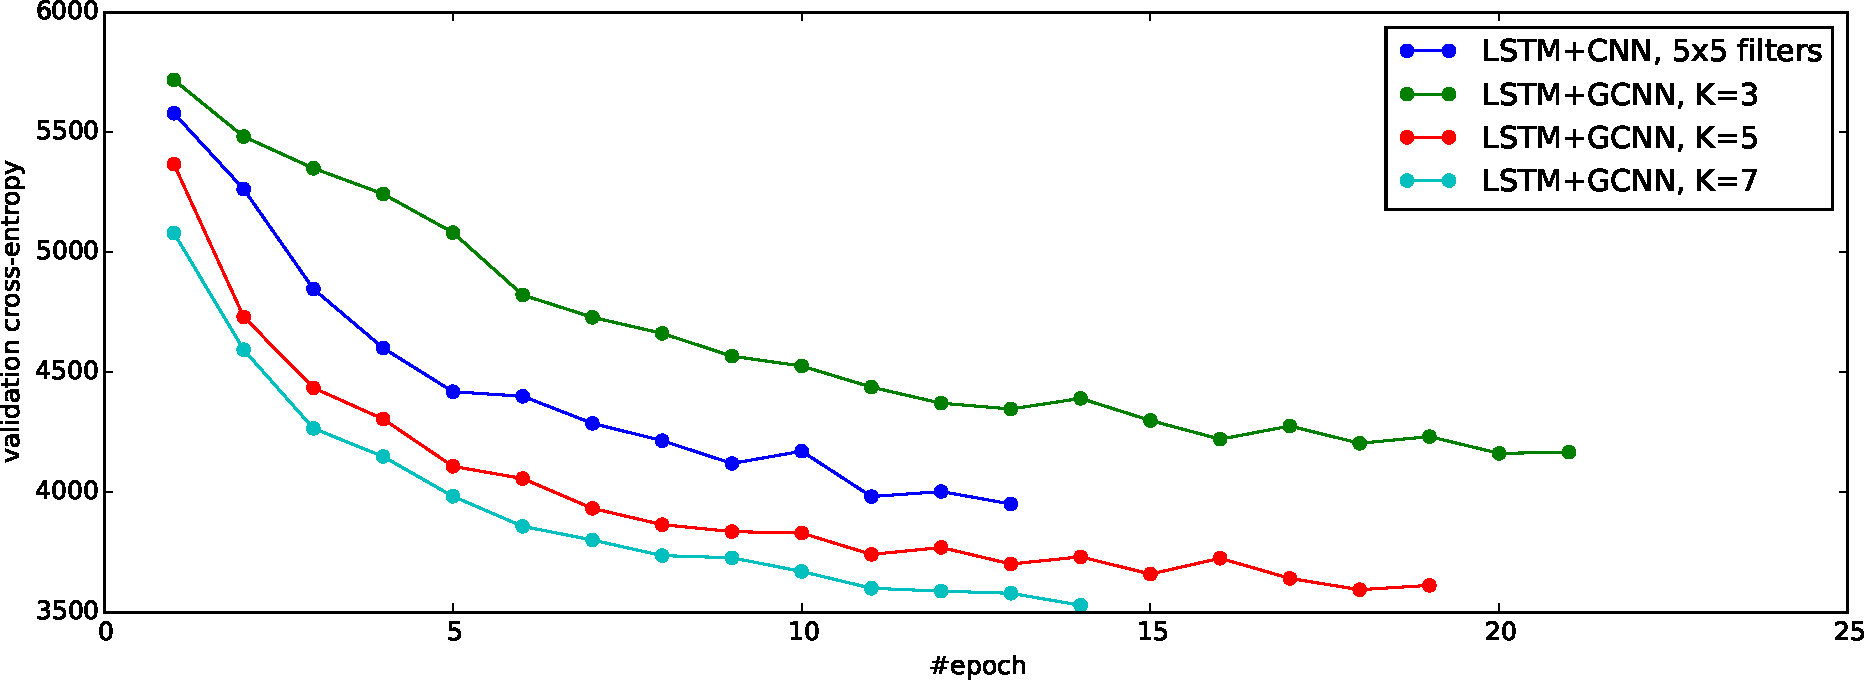
\includegraphics[width=\linewidth]{figures/moving_mnist}
%	\caption{Learning dynamic of the investigated models.}
%	\label{mMIST_graph}
%\end{figure}

\begin{figure}[ht]
	\centering
	\subfigure{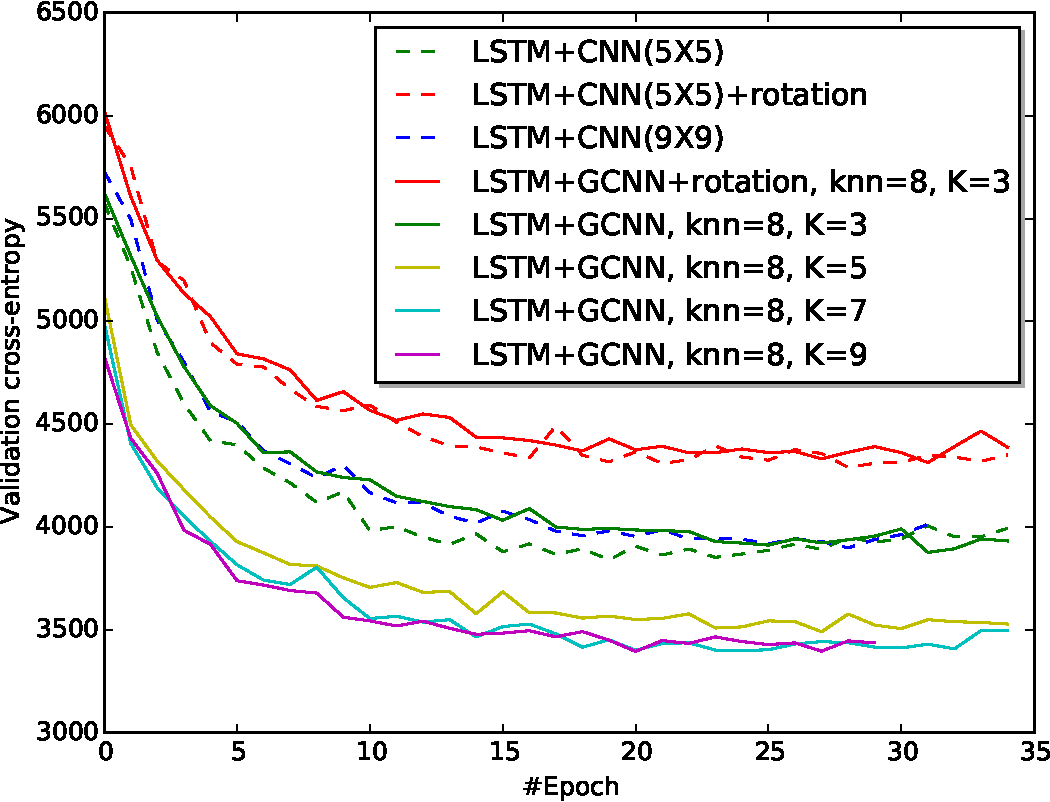
\includegraphics[width=0.48\linewidth]{figures/mMNIST_1}}
	\hfill
	\subfigure{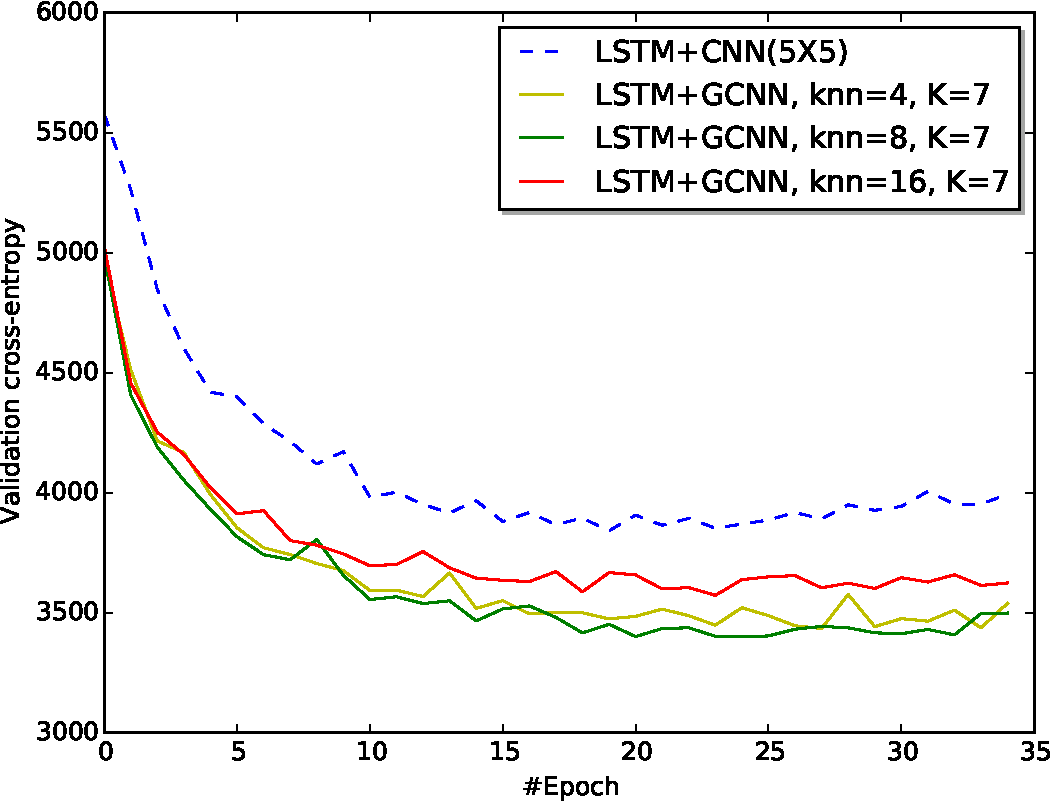
\includegraphics[width=0.48\linewidth]{figures/mMNIST_3}}
	\caption{Cross-entropy on validation set: figure on the left shows the performance of graph cnn with various size of K, while the figure on the right shows the performance changes depending on the graph structure.}
	\label{mMNIST_graph}
\end{figure}

\begin{figure}[ht]
	\centering
	\subfigure{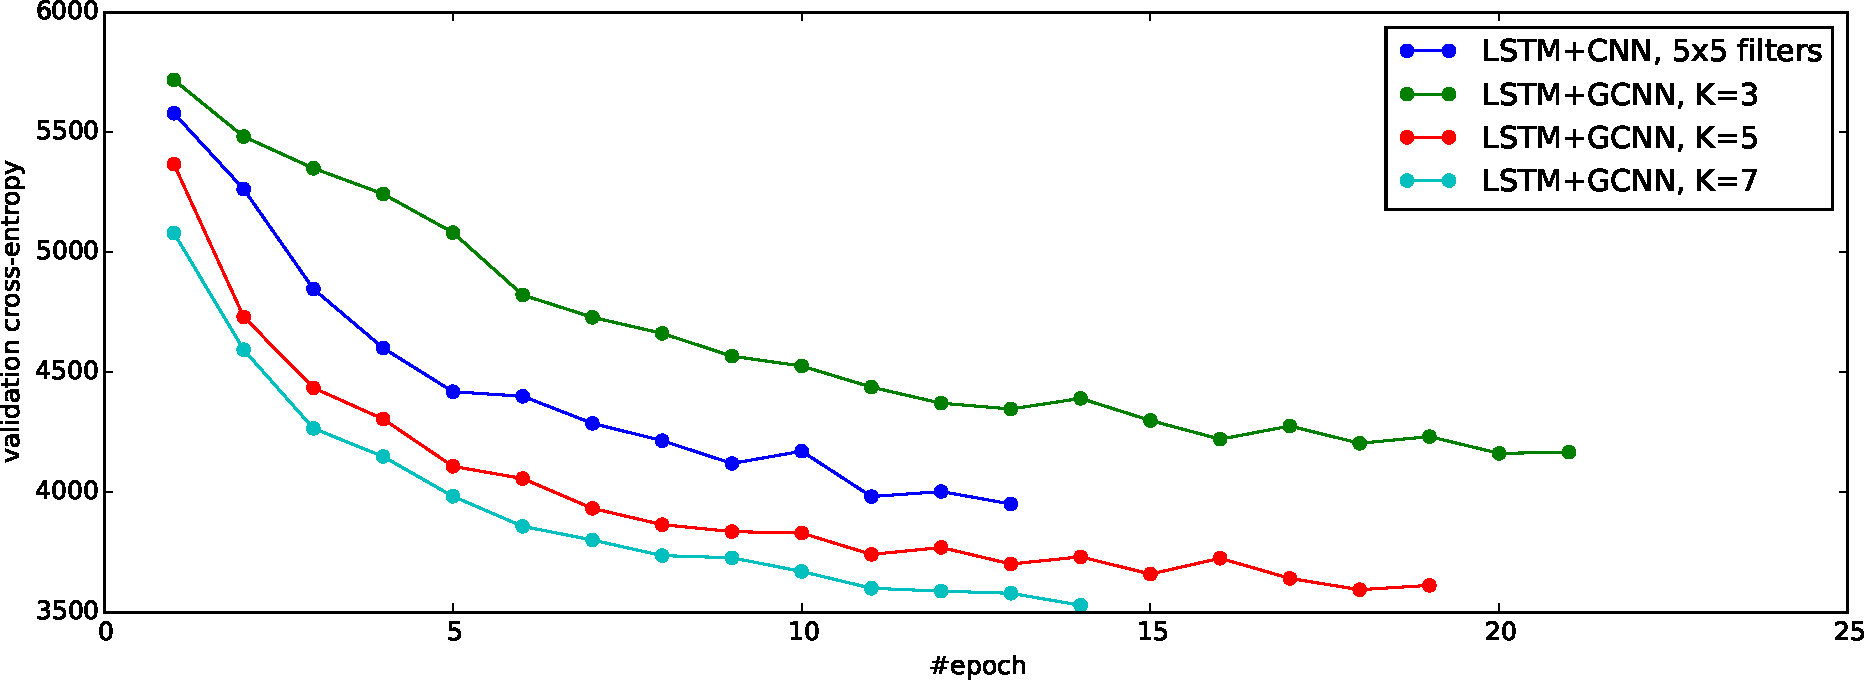
\includegraphics[width=0.9\linewidth]{figures/moving_mnist}}
	\vfill
	\subfigure{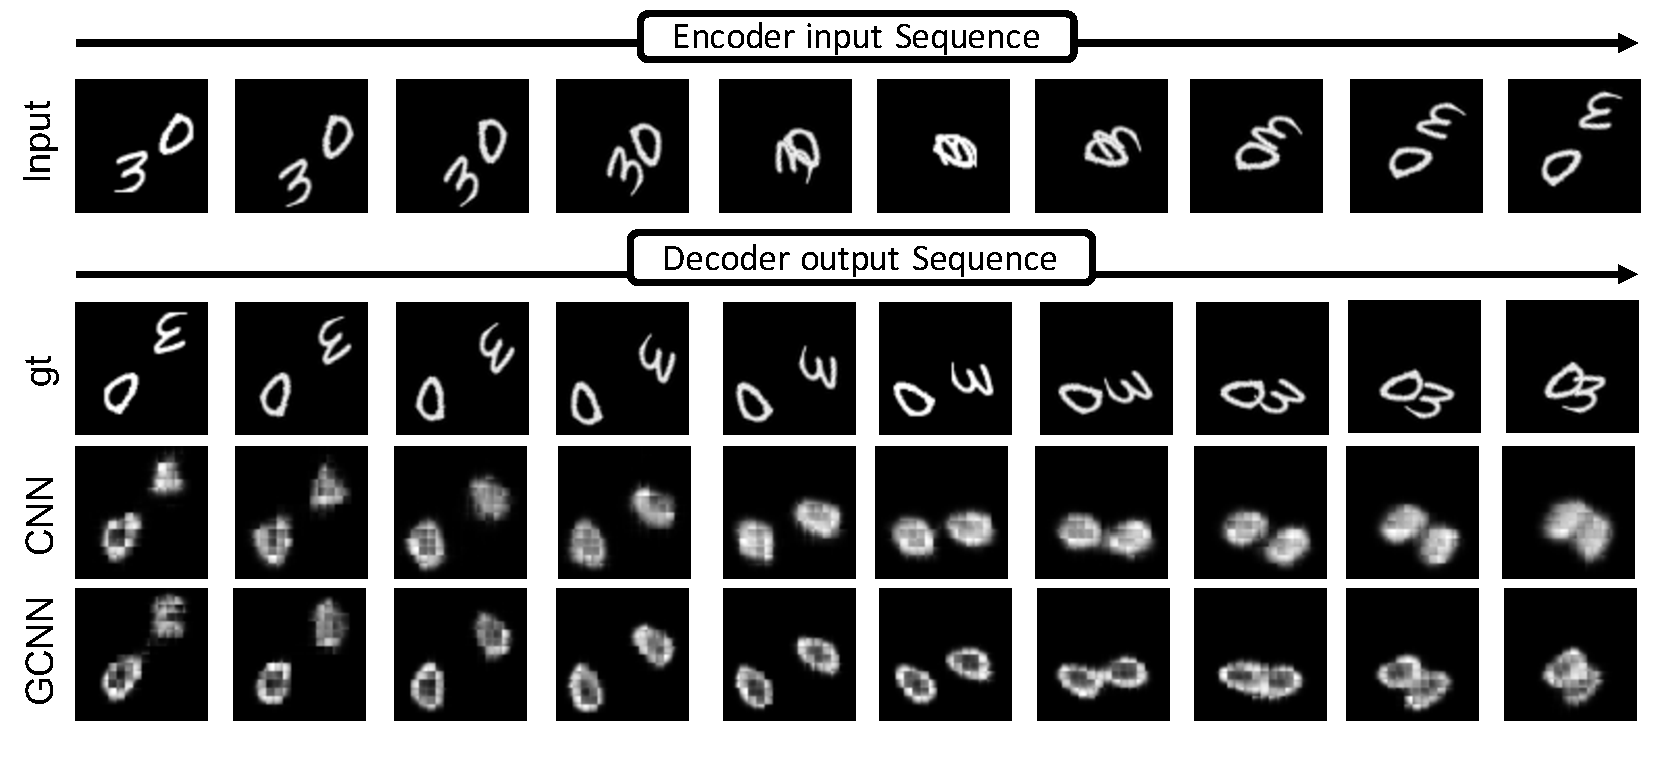
\includegraphics[width=0.9\linewidth]{figures/moving_mnist_rot}}
	\caption{Qualitative result for moving-MNIST and rotational moving-MNIST respectively. First row is the input sequence, second the ground truth and third and fourth are the predictions of the LSTM+CNN($5\times5$) and LSTM+GCNN($knn=8, K=7$)}
	\label{mMNIST_img}
\end{figure}

%\begin{figure}[ht]
%	\centering
%	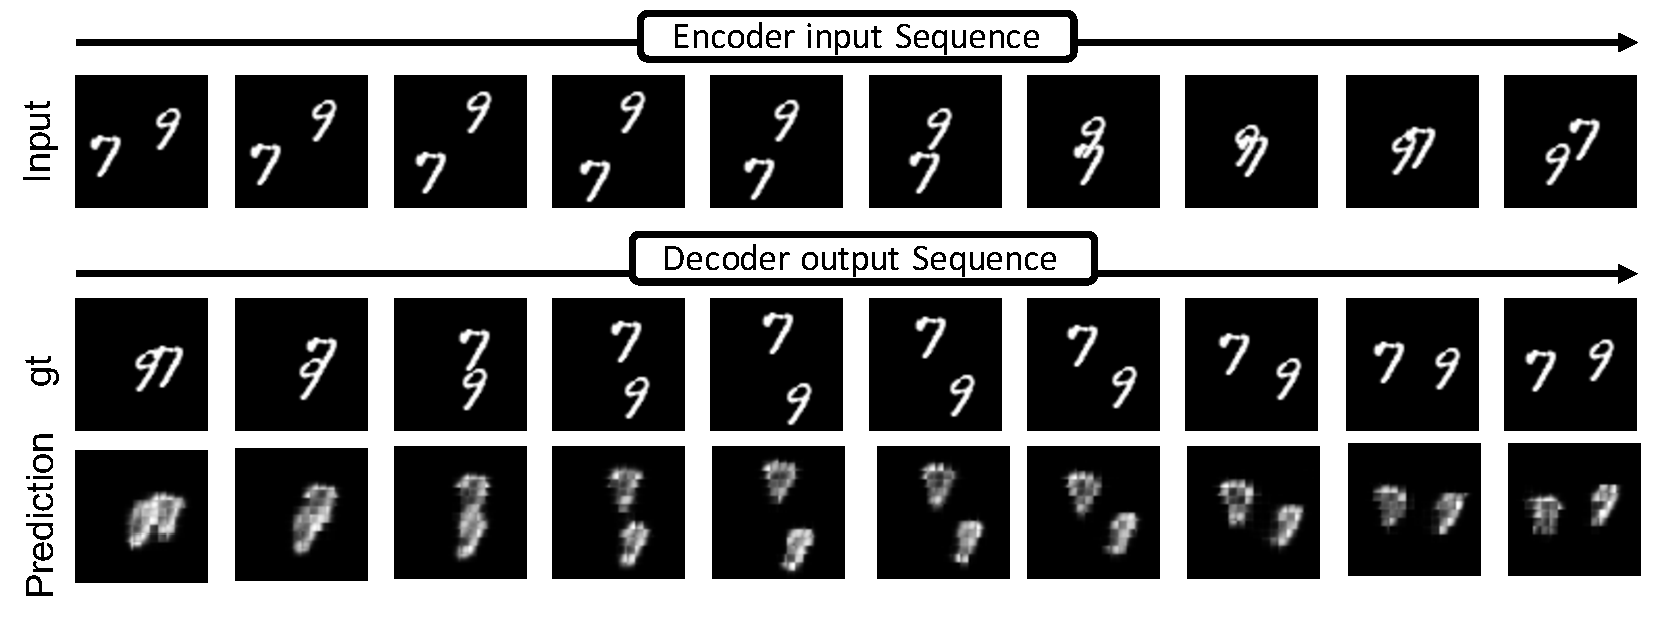
\includegraphics[width=\linewidth]{figures/result_mmnist}
%	\caption{Qualitative result for moving-MNIST. First row is the input sequence, second the ground truth and third the predictions of the 1-layer LSTM+GCNN with 8-nearest neighbor graph and $K=7$.}
%	\label{mMNIST_img}
%\end{figure}

\tabref{moving_mnist} shows the performance of various models: (i) the baseline
FC-LSTM from \citet{convlstm}, (ii) the 1-layer LSTM+CNN from \citet{convlstm}
with different filter size, and (iii) the proposed LSTM+graph CNN(GCNN) defined by \eqnref{lstm_graph_v2} with four
different values of $K$. These results show the ability of the proposed method
to capture spatio-temporal structures. Surprisingly, GCNNs can offer
better performance than regular CNNs, even when the domain is a 2D grid and the
data is images, the problem CNNs were initially developed for. One possible explanation can be the number of parameters that GCNN uses. GCNN take much less parameters than regular CNN by sharing the parameter depending on the length of the connection. Figure \ref{mMNIST_graph} on the left shows that LSTM+CNN($5\times5$) performs similar to LSTM + GCNN with $K = 3$. Because the $5\times5$ convolutional filter corresponds to $K=3$ in GCNN. However, when we increase the filter size as $9\times9$, the performance decreases because the number of parameters is increasing dramatically. Whereas GCNN can outperforms when it increases filter size to $K=7$. One another explanation can be the rotation invariance inherently provided by the graph structure. As
the nodes are not ordered, there is no notion of an edge going up, down, on the
right or on the left. All edges are treated equally. Experiment on rotational-moving MNST can explain rotation invariance property in GCNN. \tabref{moving_mnist} shows the performance gap between moving-MNST and rotational moving-MNST. LSTM+CNN($5\times5$) increases the cross-validation loss 488, whereas LSTM+GCNN($K=7$) get 403. The structure of graph also can affect the performance. Figure \ref{mMNIST_graph} on the right shows how the performance changes depending on the graph structure. We found that 8-nearest neighbor structure with K=7 performs the best on moving-MNIST. 

%\tabref{moving_mnist} shows the performance of various models: (i) the baseline
%FC-LSTM from \citet{convlstm}, (ii) the 1-layer LSTM+CNN from \citet{convlstm}
%and (iii) the proposed LSTM+GCNN defined by \eqnref{lstm_graph_v2} with three
%different values of $K$. These results show the ability of the proposed method
%to capture spatio-temporal structures. Surprisingly, graph CNNs can offer
%better performance than regular CNNs, even when the domain is a 2D grid and the
%data is images, the problem CNNs were initially developed for. An explanation
%may be the rotation invariance inherently provided by the graph structure. As
%the nodes are not ordered, there is no notion of an edge going up, down, on the
%right or on the left. All edges are treated equal.



\begin{table*}[t]
	\centering
	{\small
		\begin{tabular}{ccccccccc}
			\toprule
			LSTM Architecture & Parameters & Train Perplexity & Test Perplexity  \\
			\midrule
			\cite{zaremba2014recurrent} code\footnotemark[5] + embedding representation & 681,800 & 36.96 & 117.29 \\
			\cite{zaremba2014recurrent} code\footnotemark[5] + one-hot representation & 34,011,600 & 53.89 & 118.82 \\
			Our LSTM code + embedding representation & 681,800 & 48.38 & 120.90 \\
			Our LSTM code + one-hot representation & 34,011,600 & 54.41 & 120.16 \\
			LSTM + GCNN-M1 & 42,011,602 & 18.49 & 177.14 \\
			LSTM + one-hot + dropout  & 34,011,600 & 145.59 & 112.98 \\
			LSTM + GCNN-M1 + dropout & 42,011,602 & 114.29 & {\bf 98.67} \\
			\bottomrule
		\end{tabular}
	}
	\caption{Comparison of models in terms of perplexity. \cite{zaremba2014recurrent} code$^5$ is ran as benchmark algorithm. The original \cite{zaremba2014recurrent} code used as input representation for $x_t$ the 200-dim embedding representation of words, computed here by the gensim library$^4$. As our model runs on the original 10,000-dim one-hot representation of words, we also ran \cite{zaremba2014recurrent} code on this representation. We re-implemented \cite{zaremba2014recurrent} code with the same architecture and hyperparameters. We remind that GCNN stands for graph CNN and M1 refers to GCRN Model 1 defined in \eqnref{lstm_graph_v1}.} 
	\label{tab1}
\end{table*}


\subsection{Natural Language Modeling on Penn Treebank}



The Penn Treebank dataset has 1,036,580 words. It was pre-processed in \cite{zaremba2014recurrent} and split\footnote{\url{https://github.com/wojzaremba/lstm}} into a training set of 929k words, a validation set of 73k words, and a test set of 82k words. The size of the vocabulary of this corpus is 10,000. We use the gensim library\footnote{\url{https://radimrehurek.com/gensim/models/word2vec.html}} to compute a word2vec model \citep{word2vec} for embedding the words of the dictionary in a 200-dimensional space. Then we build the adjacency matrix of the word embedding using a 4-nearest neighbor graph with cosine distance. Figure \ref{fig2} presents the computed adjacency matrix, and its 3D visualization. We used the hyperparameters of the small configuration given by the code\footnotemark[5] based on \cite{zaremba2014recurrent}: the size of the data mini-batch is 20, the number of temporal steps to unroll is 20, the dimension of the hidden state is 200. The global learning rate is 1.0 and the norm of the gradient is bounded by 5. The learning decay function is selected to be $0.5^{\max(0,\textrm{\#epoch}-4)}$. All experiments have 13 epochs, and dropout value is 0.75. For \cite{zaremba2014recurrent}, the input representation $x_t$ can be either the 200-dim embedding vector of the word, or the 10,000-dim one-hot representation of the word. For our models, the input representation is an one-hot representation of the word. This choice allows us to use the graph structure of the words. 


\noindent
Table \ref{tab1} reports the final train and test perplexity values for each investigated model and Figure \ref{fig3} plots the perplexity value vs. the number of epochs for the train and test sets with and without dropout regularization. Numerical experiments show:
\vspace{-0.25cm}
\begin{enumerate}
\item Given the same experimental conditions in terms of architecture and {\it no} dropout regularization, the standalone model of LSTM is more accurate than LSTM using the spatial graph information ($120.16$ vs. $177.14$), extracted by graph CNN with the GCRN architecture of Model 1, Eq. \eqnref{lstm_graph_v1}. 
\item However, using dropout regularization, the graph LSTM model overcomes the standalone LSTM with perplexity values $98.67$ vs. $112.98$. 
\item The use of spatial graph information found by graph CNN speeds up the learning process, and overfits the training dataset in the absence of dropout regularization. The graph structure likely acts a constraint on the learning system that is forced to move in the space of language topics.
\item We performed the same experiments with LSTM and Model 2 defined in \eqnref{lstm_graph_v2}. Model 1 significantly outperformed Model 2, and Model 2 did worse than standalone LSTM. This bad performance may result of the large increase of dimensionality in Model 2 as the dimension of the hidden and cell states changes from 200 to 10,000, the size of the vocabulary. A solution would be to downsize the data dimensionality, as done in \cite{convlstm} in the case of image data.
\end{enumerate}












\footnotetext[5]{\url{https://github.com/tensorflow/tensorflow/blob/master/tensorflow/models/rnn/ptb/ptb\_word\_lm.py}}






%\begin{table*}[h!]
% \centering
%{\small
%\begin{tabular}{|c|c|c|c|c|c|c|c|c|}
%\hline
% LSTM Architecture & Train Perplexity & Test Perplexity  \\
%\hline
%\cite{zaremba2014recurrent} code\footnotemark[5] + embedding representation & 36.96 & 117.29 \\
%\cite{zaremba2014recurrent} code\footnotemark[5] + one-hot representation & 54.32 & 116.67 \\
%Our LSTM code + embedding representation & 48.38 & 120.90 \\
%Our LSTM code + one-hot representation & 54.41 & 120.16 \\
%LSTM + GCNN-M1 & 18.49 & 177.14 \\
%LSTM + one-hot + dropout  & 145.59 & 112.98 \\
%LSTM + GCNN-M1 + dropout & 114.29 & {\bf 98.67} \\
%\hline
%\end{tabular}
%}
%\caption{Comparison of models in terms of perplexity. \cite{zaremba2014recurrent} code$^5$ is ran as benchmark algorithm. The original \cite{zaremba2014recurrent} code used as input representation for $x_t$ the 200-dim embedding representation of words, computed here by the gensim library$^4$. As our model runs on the original 10,000-dim one-hot representation of words, we also ran \cite{zaremba2014recurrent} code on this representation. We re-implemented \cite{zaremba2014recurrent} code with the same architecture and hyperparameters. We remind that GCNN stands for graph CNN and M1 refers to GCRN Model 1 defined in \eqnref{lstm_graph_v1}.} 
%\label{tab1}
%\end{table*}



\begin{figure}[h!]
	\centering
	\subfigure[]{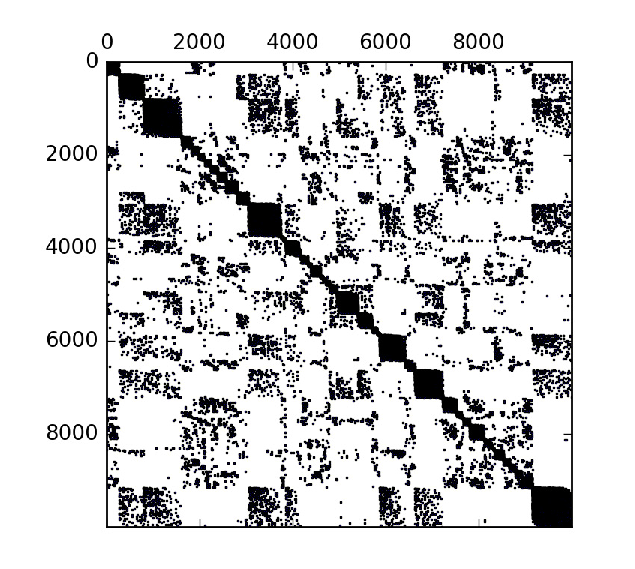
\includegraphics[height=5cm]{figures/matrixW}}
	\hspace{0.5cm}
	\subfigure[]{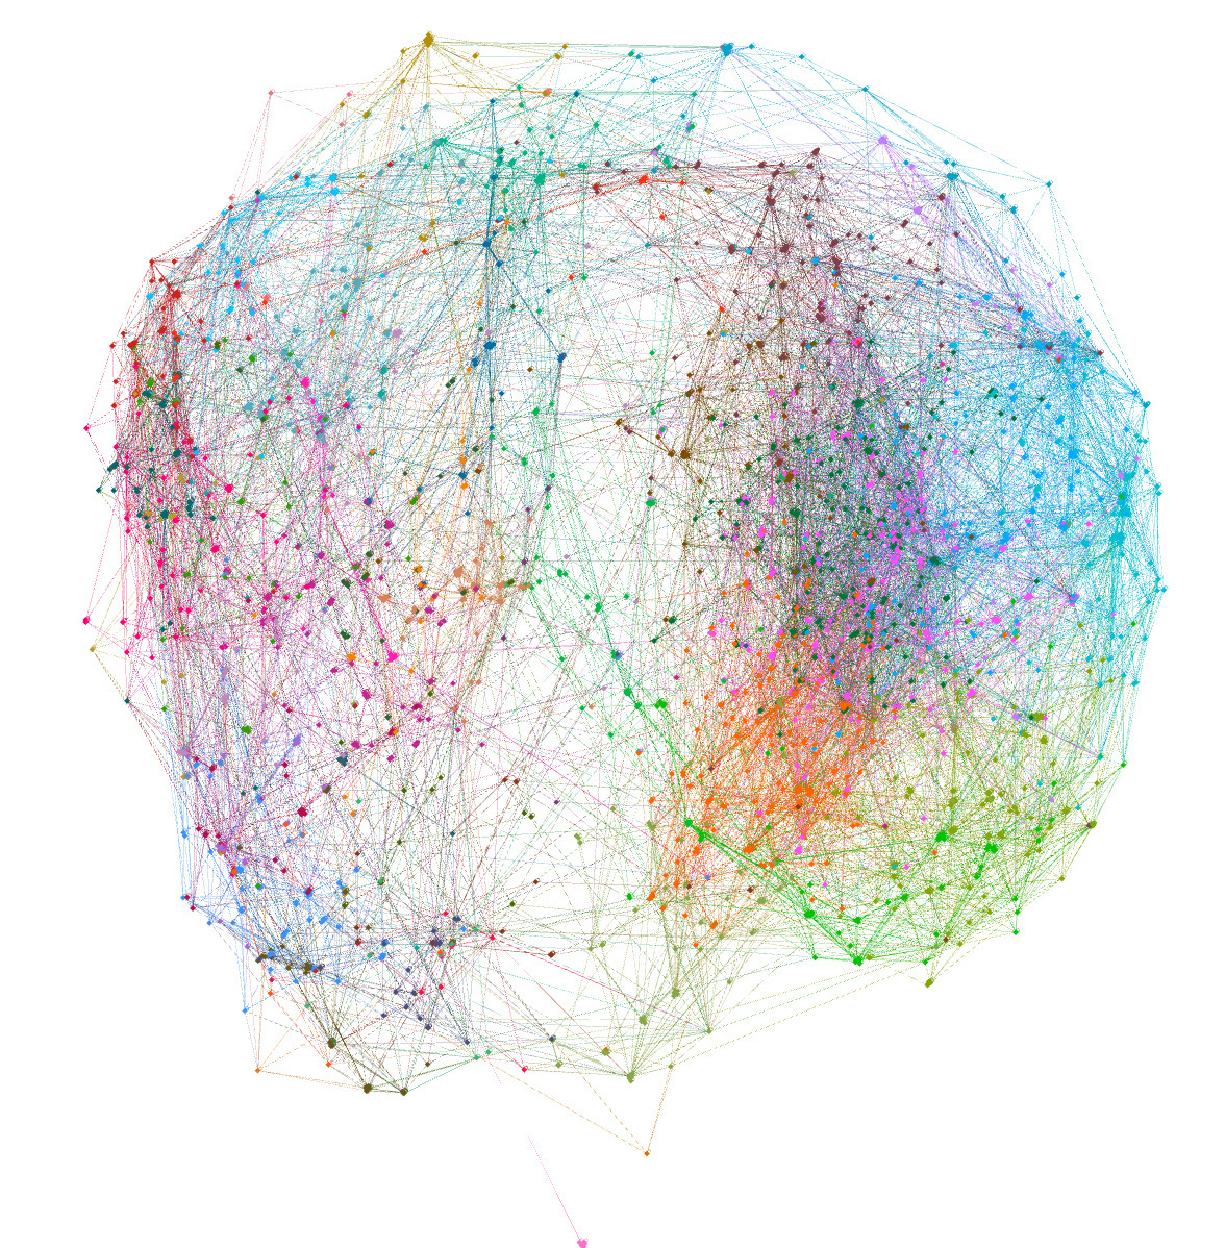
\includegraphics[height=5cm]{figures/embedding}}
	\caption{Left figure shows the adjacency matrix of word embeddings, and right figure presents a 3D visualisation of words' structure.}
	\label{fig2}
\end{figure}

\begin{figure}[h!]
	\centering
	\subfigure{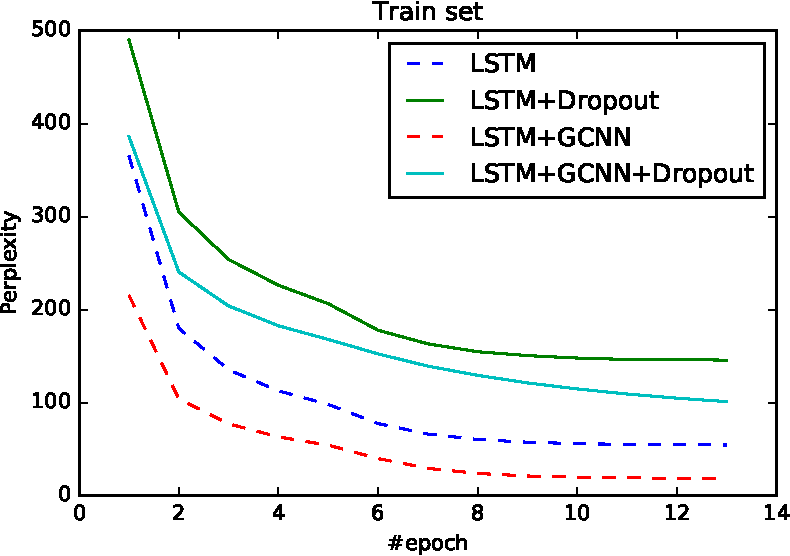
\includegraphics[width=0.48\linewidth]{figures/fig_ptb_train_small_config}}
	\hfill
	\subfigure{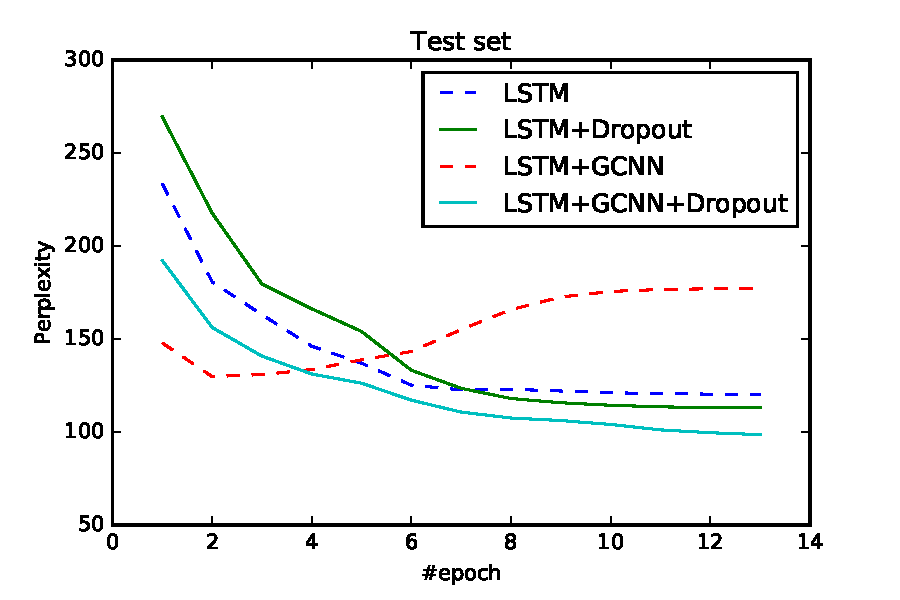
\includegraphics[width=0.48\linewidth]{figures/fig_ptb_test_small_config}}
	\caption{LSTM with and without graph information and dropout regularization: Dynamic of learning processes, that is perplexity vs. epoch for the investigated models on the training and testing sets.}
	\label{fig3}
\end{figure}







\section{Conclusion and Future Work}

This work aims at learning spatio-temporal structures from graph-structured and time-varying data. In this context, the main challenge is to identify the best possible architecture that combines simultaneously recurrent neural networks like vanilla RNN, LSTM or GRU with convolutional neural networks for graph-structured data. We have investigated here two architectures, one using a stack of CNN and RNN (Model 1), and one using convLSTM that considers convolutions instead of fully connected operations in the RNN memory (Model 2). We have then considered two applications; video prediction and natural language modeling. Model 2 has shown good performances in the case of video prediction, by improving the results of \citet{convlstm}. Model 1 has also provided promising performances in the case of language modeling, particularly in terms of learning speed. Future work will investigate applications to data naturally structured as dynamic graph signals, for instance fMRI and sensor networks. The graph CNN model we have used is rotationally-invariant and such spatial property seems quite attractive in real situations where motion is beyond translation. We will also investigate how to benefit of the fast learning property of our system to speed up language modeling models. Eventually, it will be interesting to analyze the underlying dynamical property of generic RNN architectures in the case of graphs. Graph structures may introduce stability property to RNN systems, and prevent them to express unstable dynamic behaviors.


%We introduced the Graph Convolutional Recurrent Network, an architecture
%designed to model graph-structured and time-varying data. The model is an
%extension of \citet{convlstm} which leverages recent advances in graph ConvNets
%\citep{gcnn}. Numerical experiments have shown the capability of the model
%\todo{to ...}
%We realized during this work that the evaluation of such generative models is hard as we don't have a proper cost function to evaluate the generated samples. To circumvent it, many researchers have moved to the generative adversarial networks (GANs) framework, a scheme introduced by \citet{gan} for training generative models where the goal is to fool a discriminator system that tries to separate data from the true distribution from data generated by the model. Such models are however difficult to train.
%Future works will both refine the model with advances in graph ConvNets, a recent area of interest, and apply the model to real-world problems.

\subsubsection*{Acknowledgments}
The research leading to these results has received funding from the European Union's 
H2020 Framework Programme (H2020-MSCA-ITN-2014) under grant agreement n$^{\circ}$ 642685 MacSeNet.
{
	\small
	\bibliography{iclr2017}
	\bibliographystyle{iclr2017}
}

\end{document}
